\documentclass[]{report}


\usepackage[a4paper, 
total={170mm,257mm},
left=20mm,
top=20mm,
]{geometry}

\usepackage[utf8]{inputenc}
\usepackage[portuges]{babel}
\usepackage{subcaption}
\usepackage{graphicx}
\usepackage{amsmath}
\usepackage{subfiles}
\usepackage{bm}

% Title Page
\title{Robô seguidor de linha}
\author{
	Daniel Barros\\
	\texttt{up201704271@fe.up.pt}
	\and
	Ricardo Falcão\\
	\texttt{up201704220@fe.up.pt}
}


\begin{document}
\maketitle

\section*{Introdução}
No âmbito da cadeira de SBMI, foi nos proposto o desenvolvimento de um robô seguidor de linha, utilizando para isso motores DC e sensores óticos. Neste relatório demonstraremos o nosso processo de desenvolvimento do projeto, assim como as conclusões que dele tiramos.

\section*{Arquitetura}
O robô projetado é dividido em 3 secções fundamentais: Recolha de informação, processamento dessa informação, e atuação por meio dos motores. Estas serão explicadas ao pormenor de seguida:

\subsection*{Recolha de informação}
Na recolha de informação foi utilizada um \textit{array} de 5 sensores IR, o CNY70. O esquema elétrico de cada sensor é o seguinte:

\begin{figure}[!htb]
	\centering
	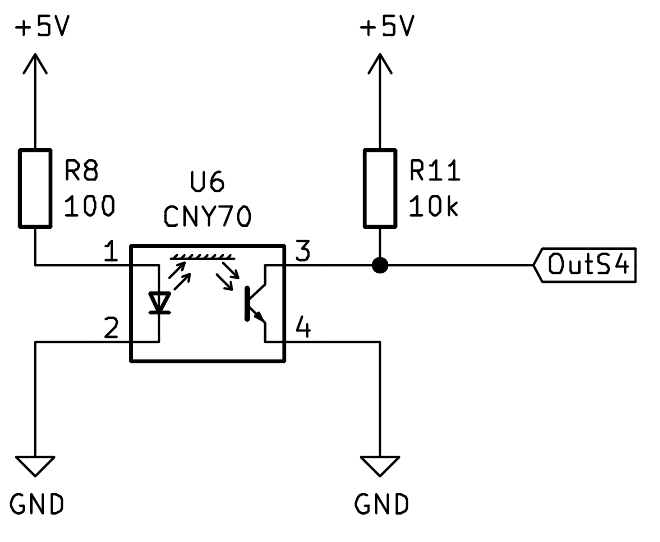
\includegraphics[width=5cm]{imagens/sensor}
	\caption{Sensores de linha (CNY70)}
\end{figure}

Perante esta configuração, era necessário uma corrente de 50 mA no LED emissor, e foi dimensionada então uma resistência limitadora de corrente de 100 $\Omega$; No coletor do foto-transístor estará uma tensão que varía com a intensidade de luz recebida. Quanto menor for a luz recebida, maior será a tensão $V_{out}$. \\
Será necessário, na pista, utilizar cores bastante diferentes no chão e na linha, para atingir a máxima resolução deste sensor. Nos nossos testes, foi utilizada uma pista de fundo branco com uma linha preta, mas o contrário era também admissível. \\
Devido ao elevado número de sinais analógicos a serem processados (que será abordado posteriormente), foi necessário utilizar um multiplexador analógico, nomeadamente o CD4051B. O seu esquema elétrico é o seguinte:

\begin{figure}[!htb]
	\centering
	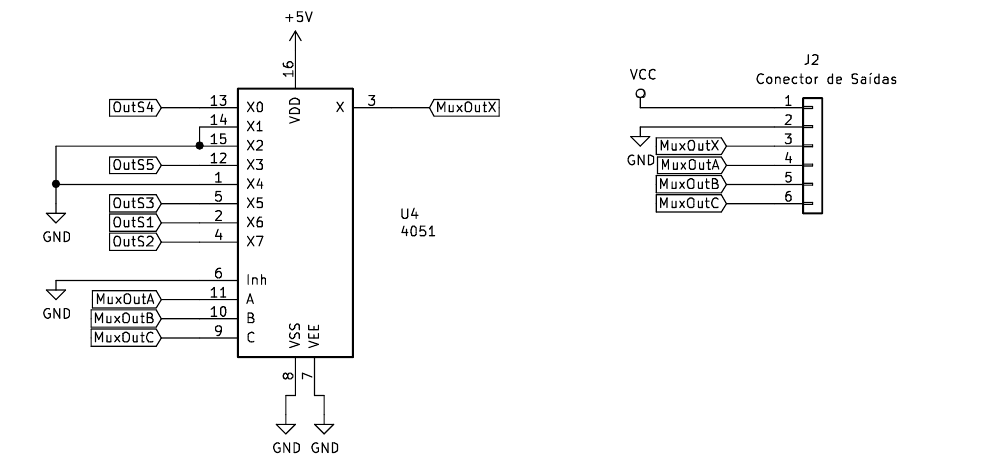
\includegraphics[width=14cm]{imagens/mux}
	\caption{Multiplexador analógico (CD4051B)}
\end{figure}

\pagebreak

\subsection*{Processamento de sinal}
Para o processamento de sinal foi utilizado o microcontrolador Atmega328p, numa placa Arduino Uno.
O processamento de sinal tem a seguinte sequência de passos:


\begin{figure}[!htb]
	\centering
	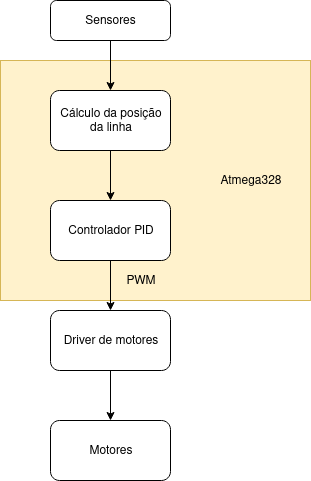
\includegraphics[width=5cm]{imagens/atmega_flow}
	\caption{Processamento de sinal (Atmega328)}
\end{figure}

Para o calculo da posição da linha é primeiro necessário ler as tensões de saída dos sensores óticos através do conversor ADC interno do microcontrolador. Estes valores devem ser calibrados no código, isto é, armazenado o menor valor lido assim como o valor máximo. Cada leitura posterior do sensor, será então transformada num número decimal, sendo 0 quando corresponde ao valor mínimo, e 1 no valor máximo. Cada leitura é amostrada 4 vezes, sendo feita a média posteriormente, para evitar erros de leitura:

\begin{equation*}
	P_x = \frac{A_{x} - A_{min}}{A_{max} - A{min}}
\end{equation*}

\vspace{1cm}

Se para cada sensor atribuirmos o seguinte peso:

\begin{table}[!htb]
	\centering
	
	\begin{tabular}{|l|l|l|l|l|}
		\hline
		\textbf{Sensor 1} & \textbf{Sensor 2} & \textbf{Sensor 3} & \textbf{Sensor 4} & \textbf{Sensor 5} \\
		1000 & 2000 & 3000 & 4000 & 5000 \\
		\hline
	\end{tabular}
\end{table}

\noindent então a média pesada destes sensores será a seguinte:

\begin{equation*}
	L_i = \frac{1000 P_1 + 2000 P_2 + 3000 P_3 + 4000 P_4 + 5000 P_5}{1000 + 2000 + 3000 + 4000 + 5000}
\end{equation*}

\begin{figure}[!htb]
	\centering
	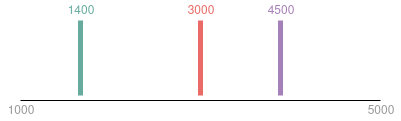
\includegraphics[width=10cm]{imagens/line}
	\caption{Algumas posições da linha}
\end{figure}

Posteriormente, este valor correspondente à posição da linha [1000;5000] é transformado numa gama de [-1;1] com a seguinte equação:

\begin{equation*}
	L = \frac{L_i - 3000}{2000}
\end{equation*}

\subsection*{Atuação dos motores}
Utilizamos dois motores de 500 RPM, assim como uma esfera metálica como terceira roda. Para o controlo destes motores era necessário utilizar um driver. Escolhemos o L298N pois permite controlar dois motores ao mesmo tempo, através de um sinal PWM, gerado no nosso microcontrolador. O esquema elétrico do driver é o  seguinte:


\begin{figure}[!htb]
	\centering
	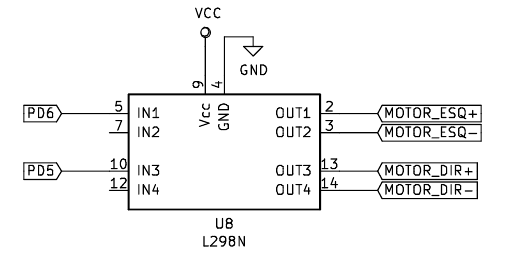
\includegraphics[width=8cm]{imagens/driver}
	\caption{Driver de motores (L298N)}
\end{figure}

Para controlar os motores, utilizamos dois sinais PWM, sendo que quanto maior for o \textit{duty cycle}, maior será a velocidade dos motores.

\subsection*{Controlo do movimento}
Com estas três componentes criamos então um sistema realimentado, como na figura seguinte:


\begin{figure}[!htb]
	\centering
	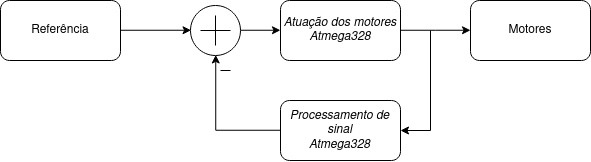
\includegraphics[height=3cm]{imagens/real}
	\caption{Sistema realimentado simples}
\end{figure}

De forma a conseguirmos um melhor controlo sobre o movimento do carro, decidimos utilizar um controlador PID. Assim, podemos não só seguir linhas retas, como também diferentes tipos de linhas curvas. Para além das três componentes do PID, utilizamos uma quarta componente, chamada constante de redução, $K_R$, que utilizamos para reduzir a velocidade do carro quando deteta uma curva.

\begin{figure}[!htb]
	\centering
	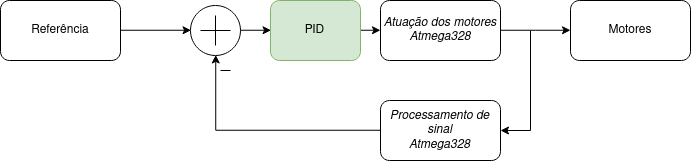
\includegraphics[height=3cm]{imagens/real_pid}
	\caption{Sistema realimentado com PID}
\end{figure}

Sendo $L$ a posição atual da linha [-1;1], e $L_o$ a posição da linha anterior, o algorítmo de controlo é o seguinte:

\begin{enumerate}
	\item $C = K_P L + K_I (L + L_o) + K_D (L_o - L)$
	\item $R = K_R (|L| + |L_o|)$
	\item $M_{esq} = v_{base} + C - R$
	\item $M_{dir} = v_{base} - C - R$
\end{enumerate}

\pagebreak

\subsection*{Componentes secundárias}
Para além da funcionalidade principal do robô seguidor de linha, implementamos umas funcionalidades extra neste projeto:

\subsubsection*{Visualizador}
Utilizamos um display OLED de 0,96 polegadas para mostrar informações sobre o estado atual do robô:

\begin{itemize}
	\item Percentagem de bateria restante
	\item Posição atual da linha (lida dos sensores)
	\item Estado do robô (Em espera, Automático)
\end{itemize}

\begin{figure}[!htb]
\centering
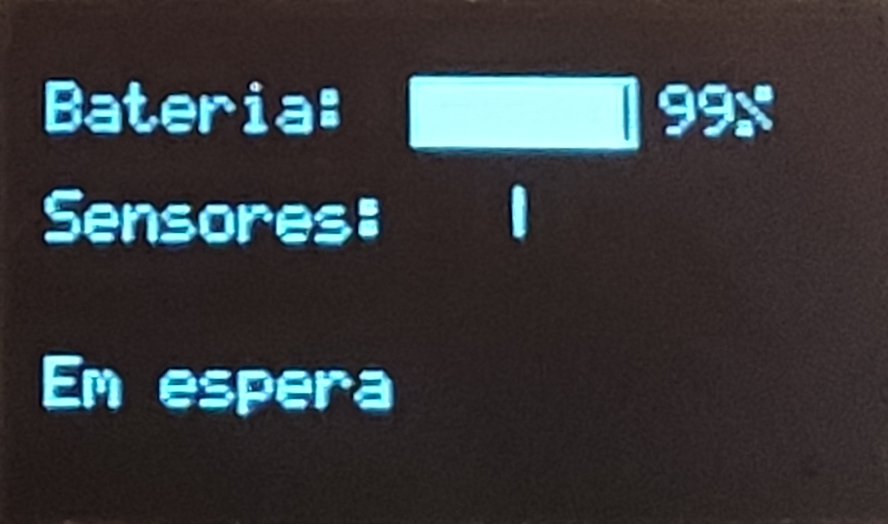
\includegraphics[width=4cm]{imagens/display}
\caption{Exemplo de um layout do visualizador}
\end{figure}

\subsubsection*{Comando remoto}
Para facilitar o desenvolvimento do robô, mas também para adicionar funcionalidade extra, utilizamos um comando de infravermelhos, assim como um recetor ligado ao microcontrolador.

\begin{figure}[!htb]
	\centering
	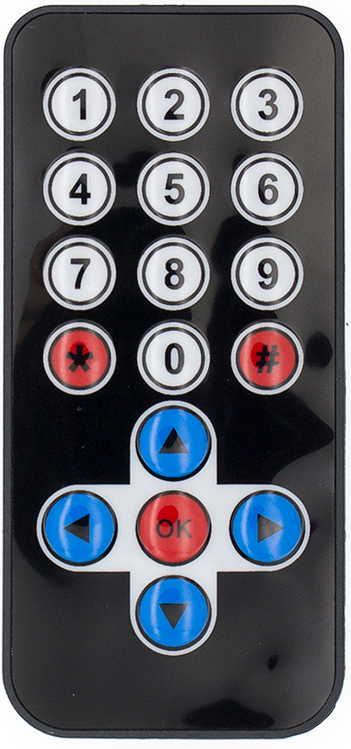
\includegraphics[width=2.5cm]{imagens/comando}
	\caption{Comando IR}
\end{figure}

\noindent Para pausar/continuar o movimento do robô é premido o botão OK. \\
As setas são utilizadas para controlar o movimento do robô quando este se encontra no modo manual.
Para iniciar o modo manual deve se premir o botão 0 quando este se encontra no estado \textit{Em espera}. \\
Os restantes números são utilizados para funções internas (calibração, velocidades).

\end{document}          
